% UACJ Thesis Template
% Program: PhD Technology
% Author: Roberto A. Contreras Masse
% Last modified on: Feb-05-2019

% Variables for thesis

\newcommand{\tituloTesis}{Titulo de la tesis}
\newcommand{\directorTesis}{Director1}
\newcommand{\coDirectorTesis}{Director2}
\newcommand{\fechaTesis}{Junio 2021}



% Specify 11pt as default font size 
% use report document class for thesis and chapters
% set up line spacing to 1.5
\documentclass[11pt]{report}
\usepackage{setspace}
\onehalfspacing

% Spanish-Mexico
% This is to use Spanish Mexico default labels for figures and tables
\usepackage[USenglish]{babel}

\usepackage{lipsum}

% Specify margins of letter paper with package geometry
\usepackage[letterpaper, top=2.5cm, bottom=2.5cm, left=3cm, right=3cm]{geometry}
% headers and footers
\usepackage{fancyhdr}
\pagestyle{fancy}
\fancyhf{}
\fancyhead[R]{\tituloTesisHeader \\ \nombreAutor}
\fancyhead[L]{}
\setlength{\headheight}{30pt}
\fancyfoot[R]{\thepage}
    \renewcommand{\headrulewidth}{0pt}
    \renewcommand{\footrulewidth}{0pt}
\fancypagestyle{plain}{
    \fancyfoot[R]{\thepage}
    \renewcommand{\headrulewidth}{0pt}
    \renewcommand{\footrulewidth}{0pt}
    }


% Use closest font to Times New Roman and enable any font size
\usepackage{mathptmx}
\usepackage{anyfontsize}

% encoding
\usepackage[utf8]{inputenc}

% Include ability to handle graphics
\usepackage{graphicx}
\graphicspath{ {images/} } % Specify images path

\usepackage{float} %设置图片浮动位置的宏包
\usepackage{subfigure} %插入多图时用子图显示的宏包




% Captions specifications
\usepackage{caption}
\captionsetup{font={small, bf}}
\newcommand\fuenteObjeto[1]{\captionsetup{font=small}\caption*{#1}}

%-------EXAMPLE----------------------------------------
% \begin{figure}
%    \centering
%    \caption{Caption}
%    \includegraphics{uacj_sinfondo_640x640.png}
%    \fuenteGrafica{fuente de la gráfica}
%    \label{fig:my_label}
% \end{figure}
%-------------------------------------------------------


% specification of chapters, sections and subsections
\usepackage{titlesec}
\titleformat{\chapter} %section to format
    {\flushleft\normalfont\fontsize{13}{14.4}\bfseries} %format
    {\thechapter.} %label 
    {12pt} %separation 
    {}
\titlespacing{\chapter}{0pt}{14pt}{0pt}

\titleformat{\section} %section to format
    {\flushleft\normalfont\fontsize{12}{12.1}\bfseries} %format
    {\thesection} %label 
    {12pt} %separation 
    {}
\titlespacing{\section}{0pt}{14pt}{0pt}

% Reference and citations

\usepackage{pdfpages}

%-------------------------------------------------------
% BEGIN MAIN DOCUMENT
%-------------------------------------------------------

\begin{document}


\begin{titlepage}

\begin{center}
    
\includegraphics[width=15cm]{images/u_logo.png} \\
    \vspace{24mm}
  
    
    {\fontsize{18}{20}
    \selectfont \textbf{Project Report for D1}} \\
    
    \vspace{8mm}             
    
    {\fontsize{14}{16}
    \selectfont SOEN 6481}
    
    {\fontsize{14}{16}
    \selectfont Software Systems Requirements Specification}
    
    {\fontsize{14}{16}
    \selectfont (2019 SUMMER)}\\
    
    \vspace{8mm}
    
    {\fontsize{18}{20}
    \selectfont \textbf{ETERNITY: NUMBERS}} \\
    
    \vspace{8mm}

    
    \vspace{8mm}
    
    {\fontsize{14}{16}
    \selectfont Zan Wang} \\
    
    
    
    \vspace{8mm}
    
    {\fontsize{12}{10} \selectfont Student ID: 27779704 } \\
    

    
\end{center}

\end{titlepage}


\tableofcontents

% Lista de tablas
% Lista de figuras

\chapter*{Abstract}
\noindent
Along with fast development of human society, it emerges lots of revolution in various territories. The development of traditional regular calculator is just one of them that is under great challenge. People are not only satisfied with the default process to obtain results from using traditional regular calculator, but desire for a more convenient and efficient solution. The widely used solution based on regular calculator with its design of scientific mode, therefore attracts lots of people’s attention. Hence, how to validate the scientific number and the scientific mathematical calculation and decent user-device interaction experience become crucial topic for calculator designer. 
To better serve to this case study here, a simple but efficient calculator design with several specific scientific calculation function with number (PI), is used to model and verify a scientific calculator. The entire case study report is organized as: after introduction, the Brief Description regarding problem 1 gives the basic background regarding the assigned number; Chapter of Interview provides the Question and Answer interview session and the interview analysis; Chapter 4, User Personas, the two interviewees are introduced and answers to problem 3 are provided; To analyze the problem domain, the concepts relationship and class diagram are provided in chapter 5 for problem 4; Problem 5 gives all the use cases and describes carefully for each. Besides, sequence diagram and activity diagram are provided for further description.

\\
%\vspace{8mm}
\begin{spacing}{1.0} 
\end{spacing} 
\noindent
{\textbf{Keywords: calculator, number, function, PI} }






\chapter{Introduction}
\noindent
This is a math/scientific calculator similar to most regular calculator in market. It supports functions for both regular calculation and scientific number calculation regarding Pi. Enter a formula by typing on the keyboard. Type in the formula as you would say it, then press = button.

\section{Functions}
\noindent
Functions can be entered by pressing the function button on the calculator. If the calculator is in scitific mode, specific scientific number PI, circular area and circular circumference could be produced by one-button press.

\section{Arithmetic Operators}
\noindent
Once you press the '=' button, the expression is evaluated according to normal algebraic operator precedence. 
$*$ Note: The three functions regarding PI will operate just by clicking one button. The exclusive thing user has to do is to input diameter which is required to calculate circulator area, circulator circumference.

\section{Memory}
\noindent
There are one memory locations you can use to store temporary results. Under it is a button labeled 'set'. When you press 'set' the current result is copied into that memory. When a memory contains a value.

\section{Automatic Features}
\noindent
If a value is preceded by pressing Circular Area Button or Circular Circumference Button, the calculator assumes you want to set this value as circular radius for calculation.

\chapter{Brief Description: Problem 1}
\vspace{8pt}
\section{Definition}
\noindent
PI is represented by the Greek letter $\Pi$ and is a constant, approximately 3.14159265 representing the ratio of the circumference to the diameter. It is an irrational number, that is, infinite loops.
\section{Practice and History}
\noindent
Calculating the value of the PI has its special meaning. However, PI with accuracy of dozens digits used in the field of modern technology are sufficient. If the size of the observable universe is calculated with a 39-degree precision PI value, the error is less than the volume of one atom. Previous people calculated PI to find out whether the PI is a circular fraction. Since 1761, Lambert proved that PI is irrational. Then in 1882, Lindeman proved that PI is the transcendental number, and the mystery of the PI is unveiled.
\section{Others}
\noindent
Besides, in 2009, the US House of Representatives formally adopted a non-binding resolution, setting March 14th of each year as the “PI-day”.
\section{Mathematical Expression}
\noindent
In the project, to realize some special scientific calculation, the Maclaurin series arcsin$($x$)$ expression will be used to approach $\pi$.
\vspace{4pt}

$\pi$$=2*(1+1/3+2/(3*5)+(3*2)/(3*5*7))+(4*3*2)/(3*5*7*9)+......)$

\\
\vspace{4pt}
\noindent
Besides, the designed calculator will use $\pi$ to complete two frequently used relevant mathematical expression:

\\
\vspace{4pt}
\noindent
1) to calculate circular circumference

$S = $\pi$r^2$

\\
\vspace{4pt}
\noindent
2) to have circular area

$C = 2$\pi$r
\chapter{Interview: Problem 2}
\vspace{8pt}

\section{Session of Question and Answer}
 \begin{itemize}

\item[1)] Do you need to deal with numbers frequently?
\item[-]Answer 1: Yes
\item[-] Answer 2: Sure 

\item[2)]How often do you use a calculator?
\item[-]Answer 1: Very often, but just some very easy calculation
\item[-]Answer 2: Sure...unless I must use my head

\item[3)]When and where do you use it?
\item[-]Answer 1: Actually, mostly I could satisfy my needs by heart work, but I choose to use calculator finally.
\item[-]Answer 2: Everywhere, all the time.

\item[4)]Do you have any personal preference for using a calculator?
\item[-]Answer 1: Yes, I like using a calculator with everything big for mutual interaction. I think that would be much more handy.
\item[-]Answer 2: I am OK with most designs for today's calculators.


\item[5)]If there is calculator, what kind of appearance would you like, say, the operators, keys, the button, the screen etc.?
\item[-]Answer 1: I hope it could be as big as my pocket, the buttons are no need to big but large screen. The operators no need to be very rich as I just need it to do some simple calculation like sum, substation, mod or multiplication. 
\item[-]Answer 2: not too big, easy to take, big screen with simple and clear buttons. For operators, four arithmetic operation is enough for me.


\item[6)]what do you think is the most necessary function with PI involved in this device?
\item[-]Answer 1: as I mentioned previously, circumference and area are often used, so I hope it has one-button circumference or area calculation function.
\item[-]Answer 2: to calculate circle area which is highly desired for me.


\item[7)]When you use the function, what other parameters do you think you are going to use?
\item[-]Answer 1: input radius or diameter, get circumference and area
\item[-]Answer 2: it is better to be able to record a group of parameter or numbers, so I can just find them in machine memory but no need to recall in head.

\item[8)]If the function is created, do you think what is the best way for you to use it conveniently?
\item[-]Answer 1: One-button calculations!
\item[-]Answer 2: Speech control perhaps...I don't want to type numbers all the time.

\end{itemize}

\section{Analysis}
\vspace{8pt}
\noindent
This interview gives an overview of  the expectation of two potential users for a calculator with a special number.  The interview was conducted with one domain professional and one common user.\\
 \hfill\break
Firstly, calculators are still broadly used, even for today with rapid development of technology, general-purpose calculators still have a very wide range of users.\\
 \hfill\break
Second, in addition to the desire for a more portable and easy-to-use design, it is also desirable to incorporate new technologies such as speech recognition.\\
 \hfill\break
Third, for special numbers, users are not satisfied with the function only to obtain the value itself, but hope to extract the calculation results related to other most used function employing a specific special number. For example, when the value of the PI is obtained, one button can also be used to obtain values of the circumference length and the circle area with PI.
\chapter{User Personas: Problem 3}
\vspace{6pt}

\section{Definition}
\vspace{4pt}
\noindent
Persona gives meaningful archetypes which we can use to assess our design development against. 
Personas are actually fictional characters, which we create based upon our research in order to represent the different user types that might use our service, product, site, or brand in a similar way. Creating personas will help us to understand our users’ needs, experiences, behaviors and goals.

\\
\vspace{4pt}
\noindent
\begin{flushleft} 

Constructing personas will help us ask the right questions and answer those questions in line with the users we are designing for. Creating personas can help we step out of ourselves. It can help us to recognize that different people have different needs and expectations, and it can also help us to identify with the user we’re designing for. Personas make the design task at hand less complex, they guide our idea processes, and they can help we to achieve the goal of creating a good user experience for our target user group.
\end{flushleft} 
\\
\vspace{4pt}
\noindent
\begin{flushleft} 
As opposed to designing products, services, and solutions based upon the preferences of the design team, it has become standard practice within many human centered design disciplines to collate research and personify certain trends and patterns in the data as personas. Hence, personas do not describe real people, but we compose our personas based on real data collected from multiple individuals. Personas add the human touch to what would largely remain cold facts in our research. When we create persona profiles of typical or atypical (extreme) users, it will help we to understand patterns in our research, which synthesizes the types of people we seek to design for. Personas are also known as model characters or composite characters.
\end{flushleft} 
\section{Information}
\vspace{4pt}
\noindent
I have interviews with two representative users. One is a professional expert whose name is Leon Gannt, the other, Mr. David Huang, is an ordinary user. Their persona information are shown as follows.



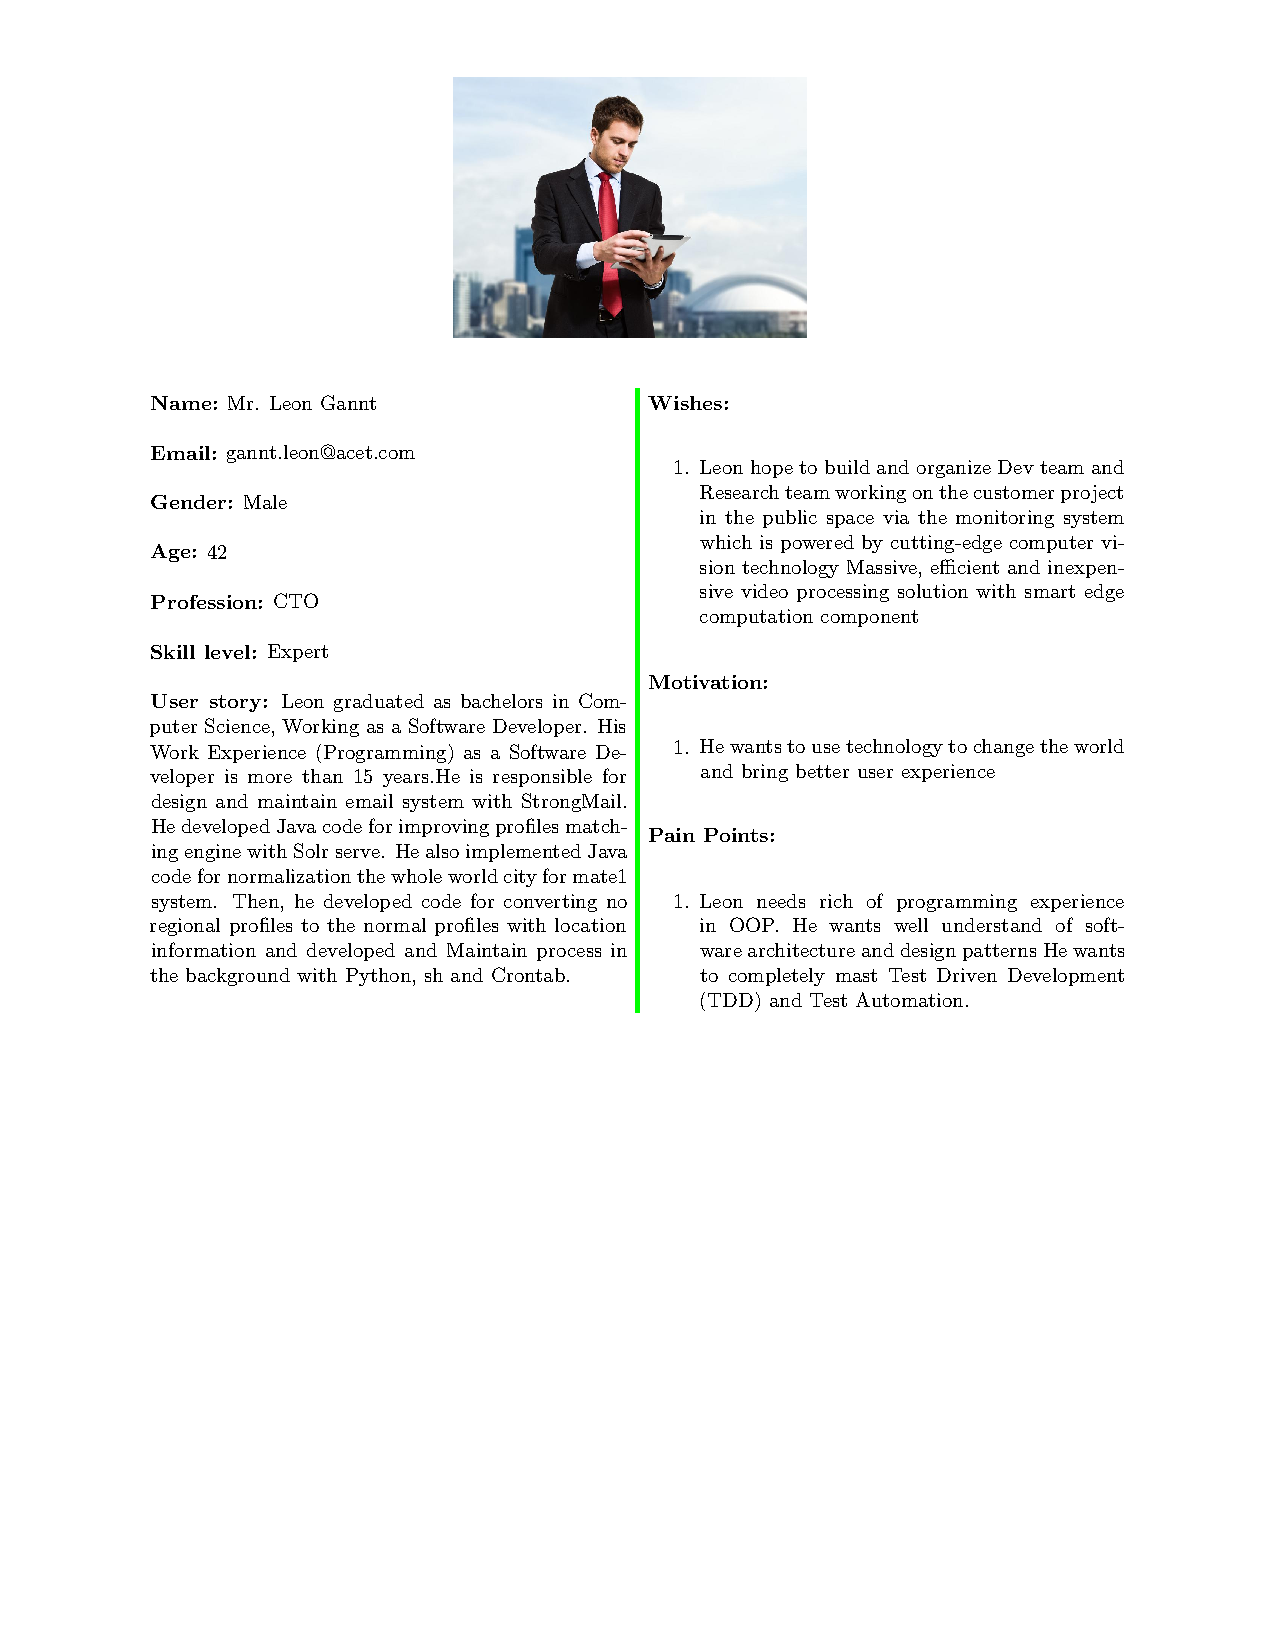
\includepdf[pages=1, scale=1]{images/1.pdf}
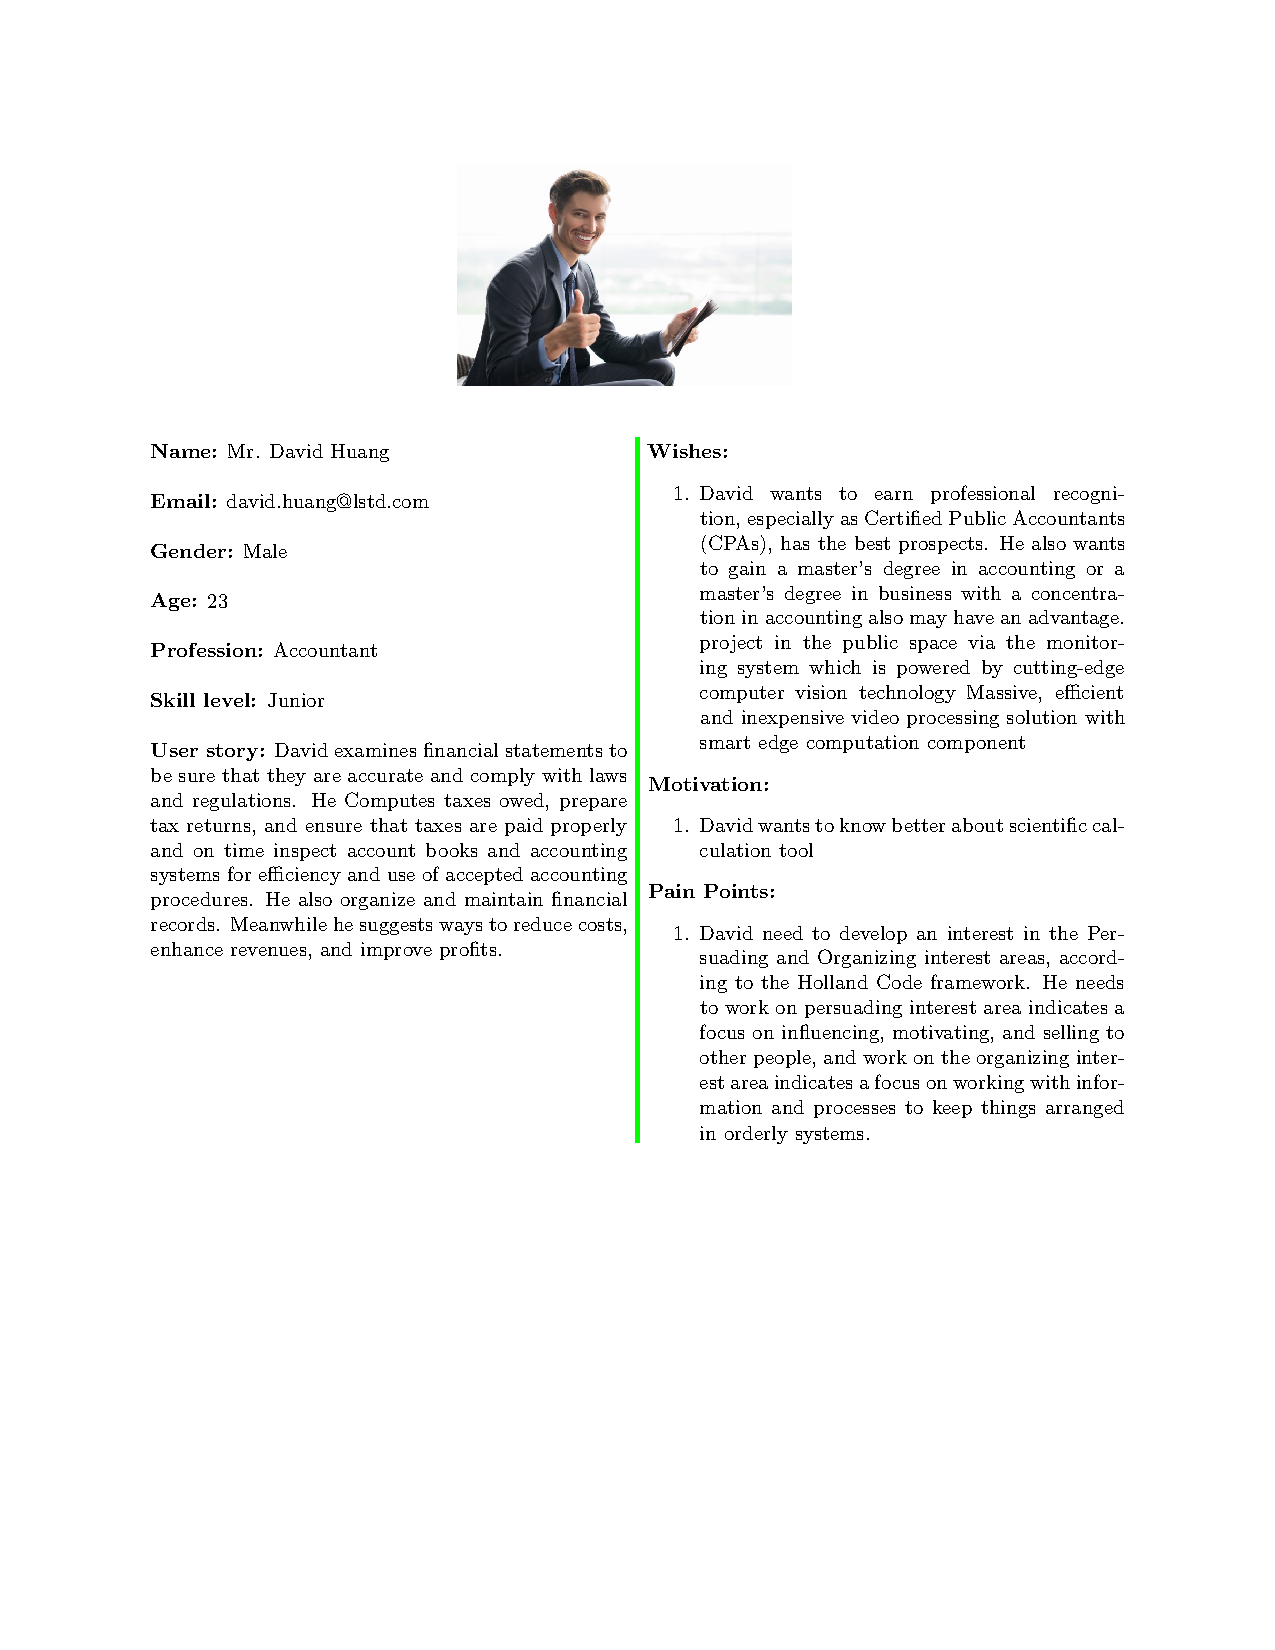
\includepdf[pages=1, scale=1]{images/2.pdf}

% \centering  %图片全局居中
% \includegraphics[width=0.9\linewidth]{images/Persona_1.pdf}


% \section{Junior}
% \centering  %图片全局居中
% \includegraphics[width=0.9\linewidth]{images/Persona_2.pdf}



























\chapter{Problem Domain: Problem 4}
\vspace{8pt}

\section{Domain Diagram}

\begin{figure}[H]
\centering  %图片全局居中

\label{Fig.sub.1}
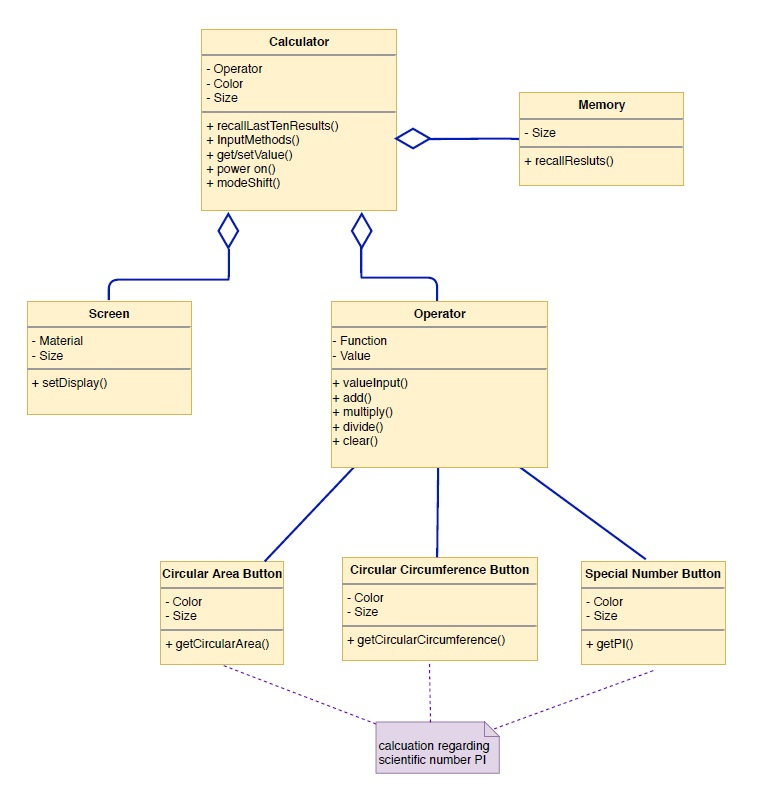
\includegraphics[width=1\textwidth]{images/class_diagram.jpg}
\caption{Domain Model}
\label{Fig.main}
\end{figure}
\vspace{50pt}

\section{Concept Relationship}

\begin{flushleft} 

\vspace{5pt}
\noindent
1)	Concepts:\\
calculator, screen, operator, memory, special number button, circular area button, circular circumference button

\vspace{8pt}
\\
\noindent
2)	Relationship:\\
screen ----------$<$$>$ calculator (aggregate relationship)
\\
operator ----------$<$$>$ calculator (aggregate relationship)
\\
memory ----------$<$$>$ calculator (aggregate relationship)

\\
special number button ----------- operator (association relationship)
\\
circular area button ------------- operator (association relationship)
\\
circular circumference button ------------- operator (association relationship)


\end{flushleft}
\chapter{Use Case Analysis : Problem 5}
\vspace{8pt}

\section{Use Cases List}

\begin{flushleft}

\vspace{5pt}
\noindent
1)	Calculate regular number: user switch on calculator, the regular number calculation mode starts by default.
\vspace{4pt}
\leavevmode\\
\noindent
2)	Input regular number: user types intended number and operators
\vspace{4pt}
\leavevmode\\
\noindent
3)	Recall last 10 results: user recollects historical 10 calculation results
\vspace{4pt}
\leavevmode\\
\noindent
4)	Calculate special number: the special number calculation mode starts by default.
\vspace{4pt}
\leavevmode\\
\noindent
5)	Get PI: user gets approximate number of PI directly
\vspace{4pt}
\leavevmode\\
\noindent
6)	Calculate circular area: user gets approximate circular area result regarding input radius using PI
\vspace{4pt}
\leavevmode\\
\noindent
7)	Calculate circular circumference: user gets approximate circular circumference regarding input radius using PI
\vspace{4pt}
\leavevmode\\
\noindent
8)	Input radius value: user type numerical value of radius for a targeted circular
\leavevmode\\

\end{flushleft}

\section{Use Cases Diagram & Description}

\begin{figure}[H]
\centering  %图片全局居中
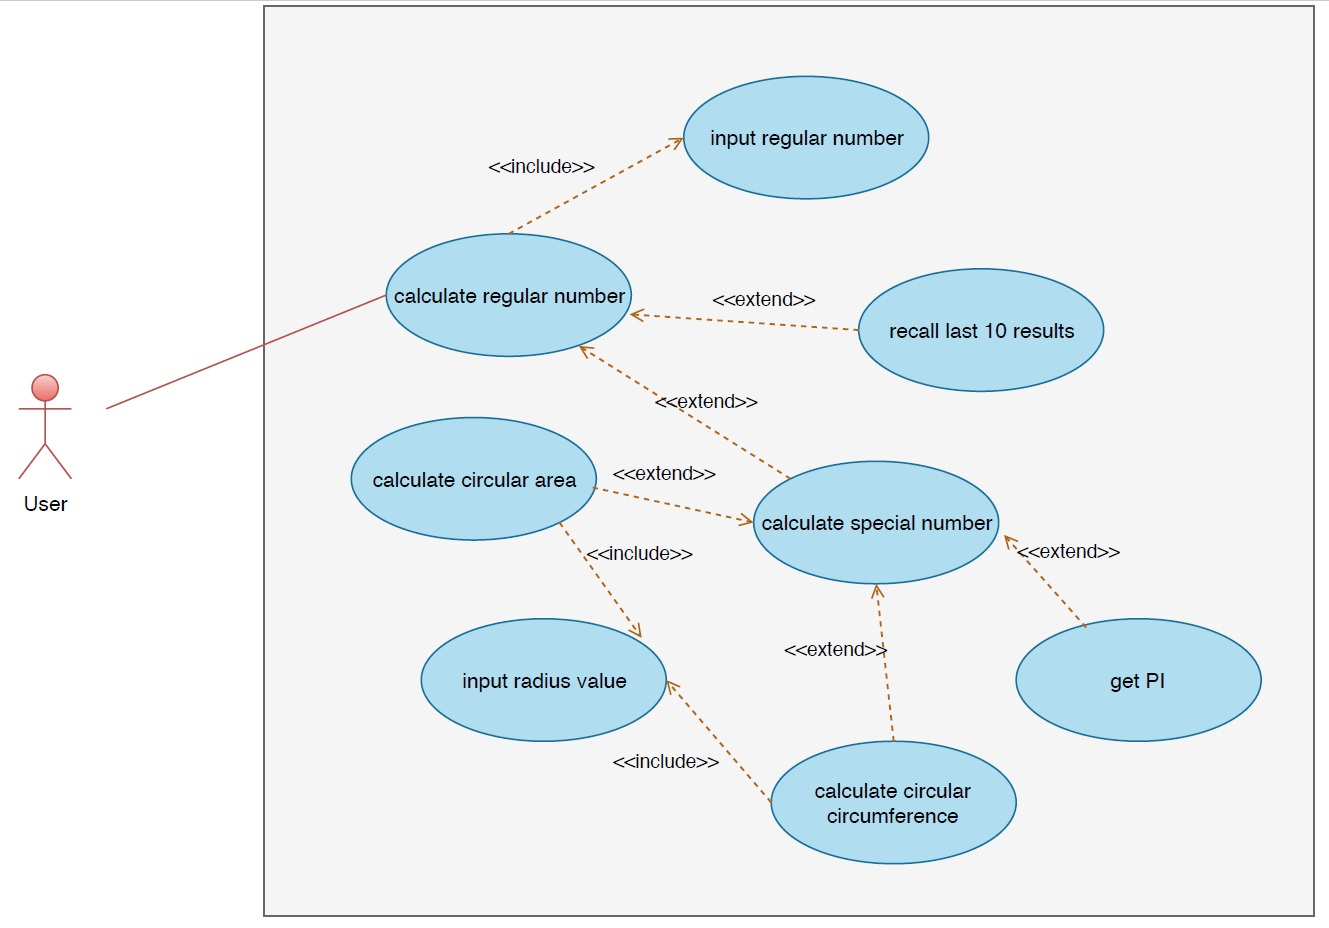
\includegraphics[width=0.9\textwidth]{images/use_case_for_all.jpg}
\caption{Use Case Diagram}
\end{figure}


\begin{figure}[H]
\centering  %图片全局居中
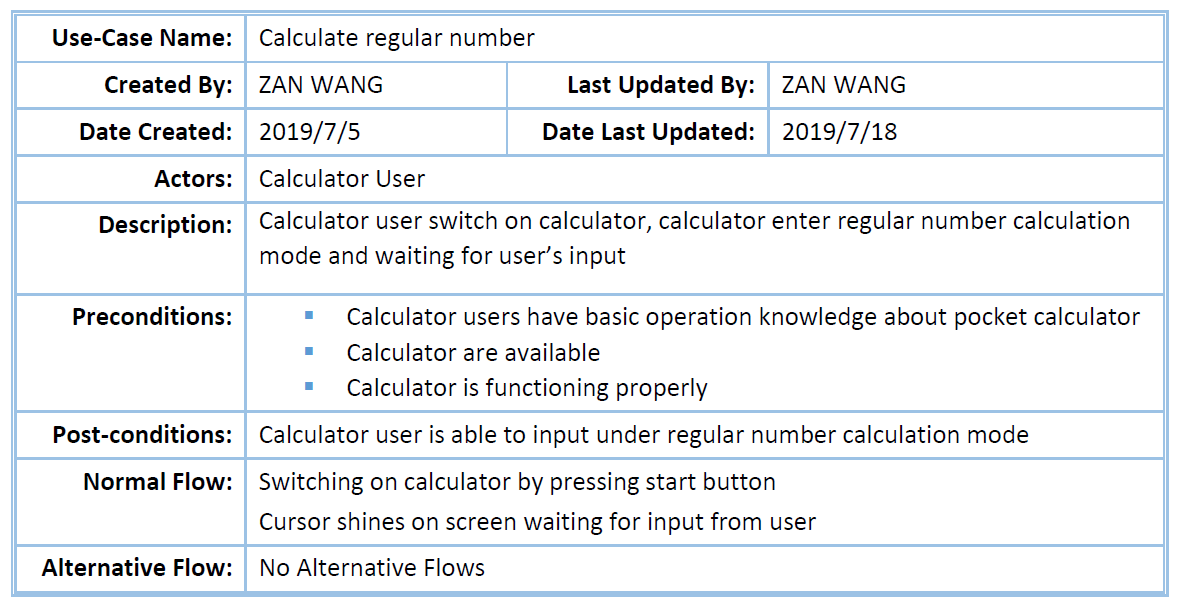
\includegraphics[width=0.9\textwidth]{images/use_case/UC_crn.PNG}
\end{figure}

\begin{figure}[H]
\centering  %图片全局居中
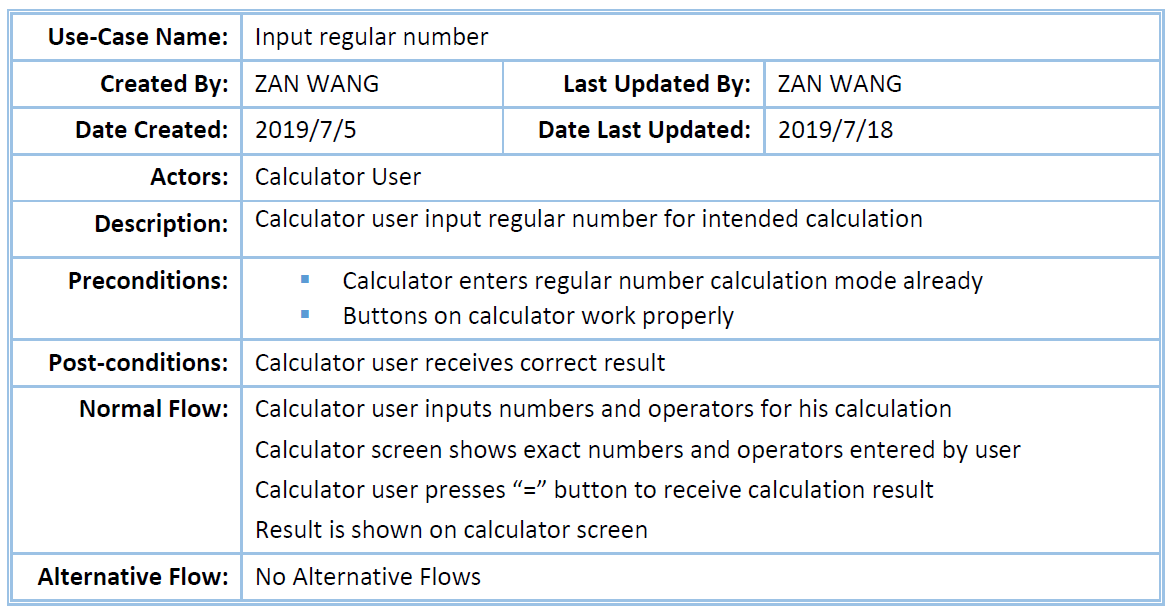
\includegraphics[width=0.9\textwidth]{images/use_case/UC_irn.PNG}
\end{figure}


\begin{figure}[H]
\centering  %图片全局居中
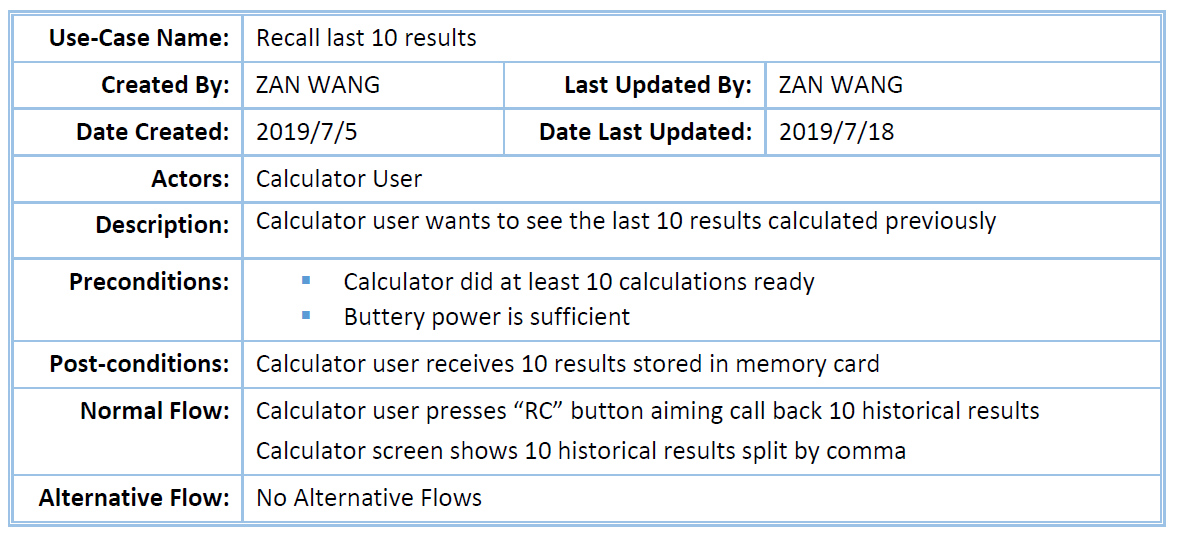
\includegraphics[width=0.9\textwidth]{images/use_case/UC_rl10r.PNG}
\end{figure}

\begin{figure}[H]
\centering  %图片全局居中
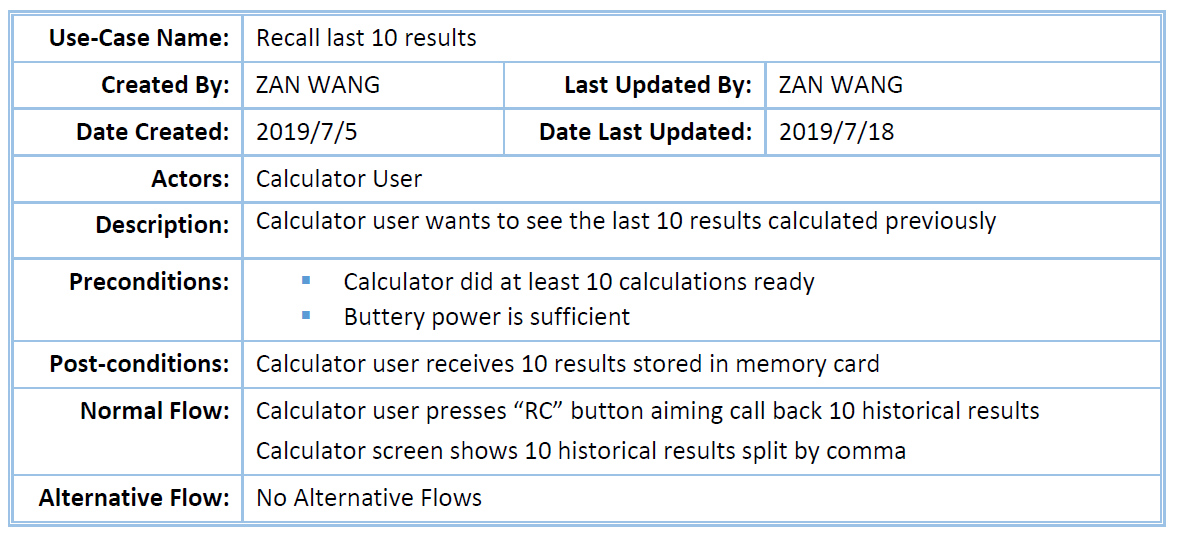
\includegraphics[width=0.9\textwidth]{images/use_case/UC_rl10r.PNG}
\end{figure}

\begin{figure}[H]
\centering  %图片全局居中
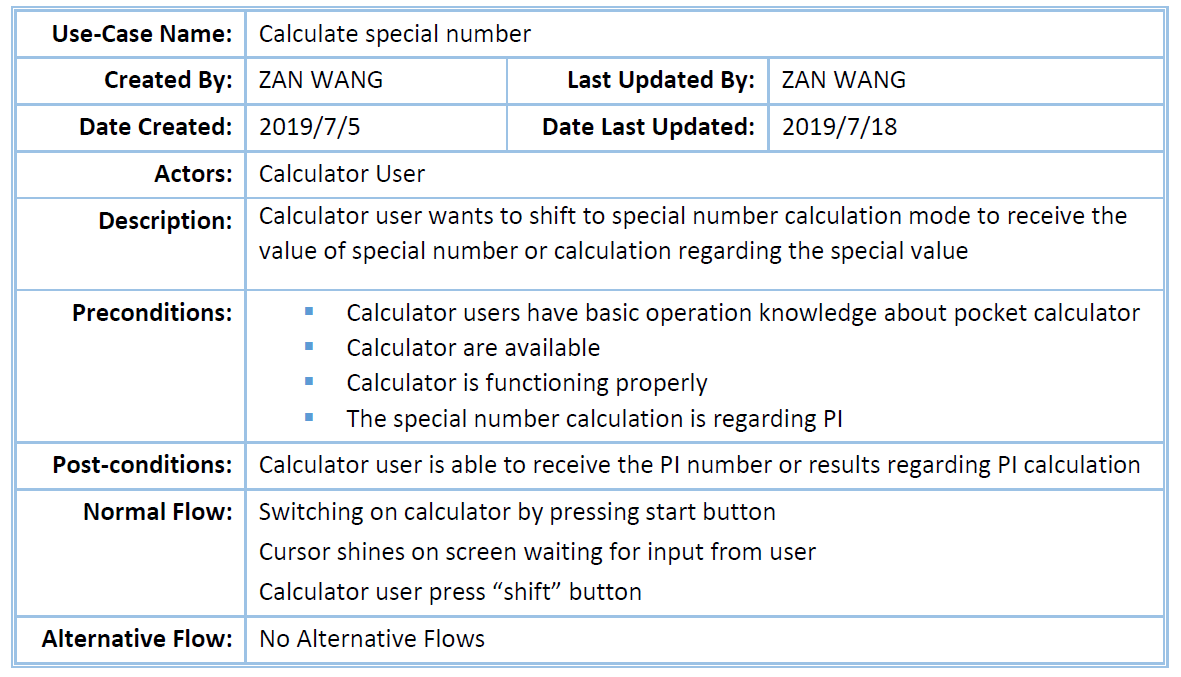
\includegraphics[width=0.9\textwidth]{images/use_case/UC_csn.PNG}
\end{figure}

\begin{figure}[H]
\centering  %图片全局居中
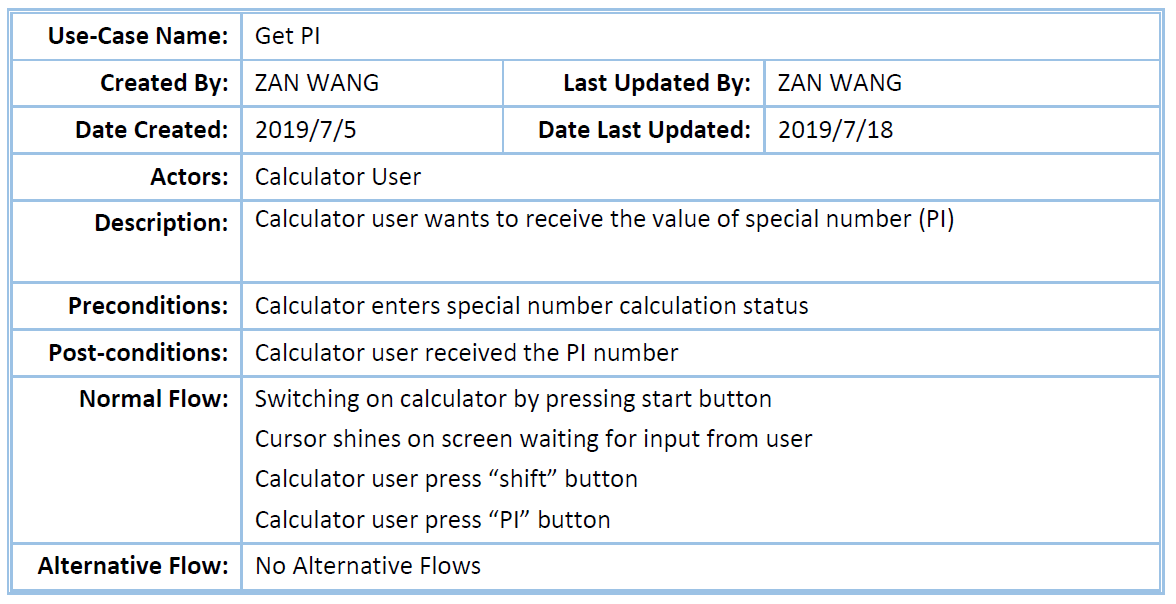
\includegraphics[width=0.9\textwidth]{images/use_case/UC_get_pi.PNG}
\end{figure}


\begin{figure}[H]
\centering  %图片全局居中
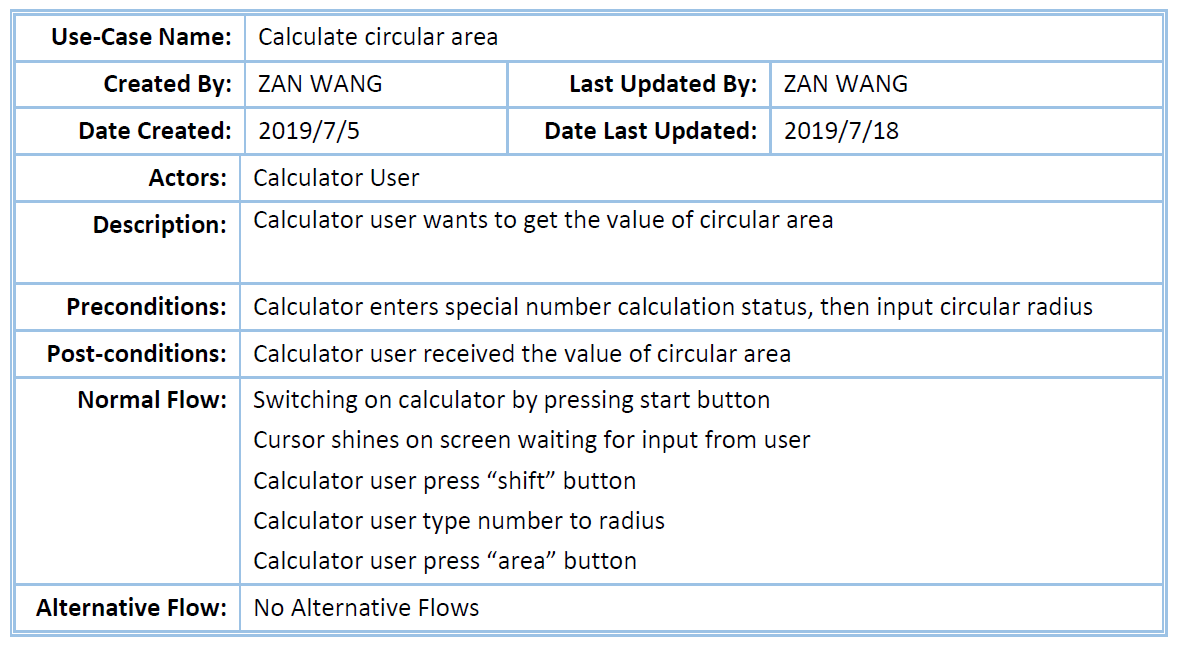
\includegraphics[width=0.9\textwidth]{images/use_case/UC_cca.PNG}
\end{figure}

\begin{figure}[H]
\centering  %图片全局居中
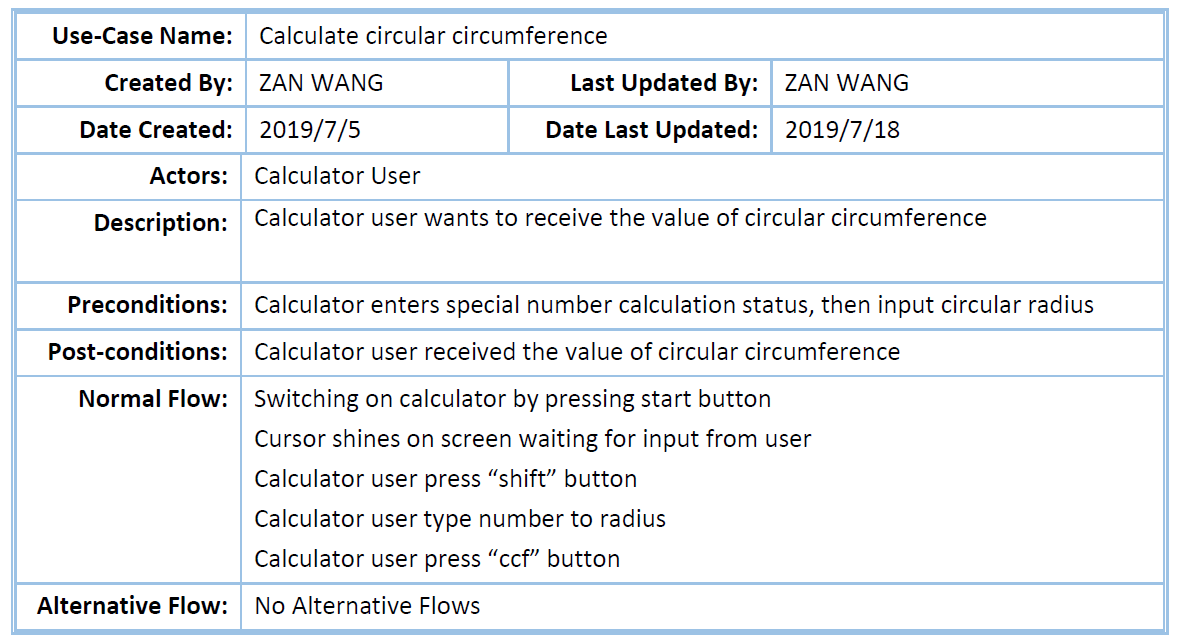
\includegraphics[width=0.9\textwidth]{images/use_case/UC_ccc.PNG}
\end{figure}

\begin{figure}[H]
\centering  %图片全局居中
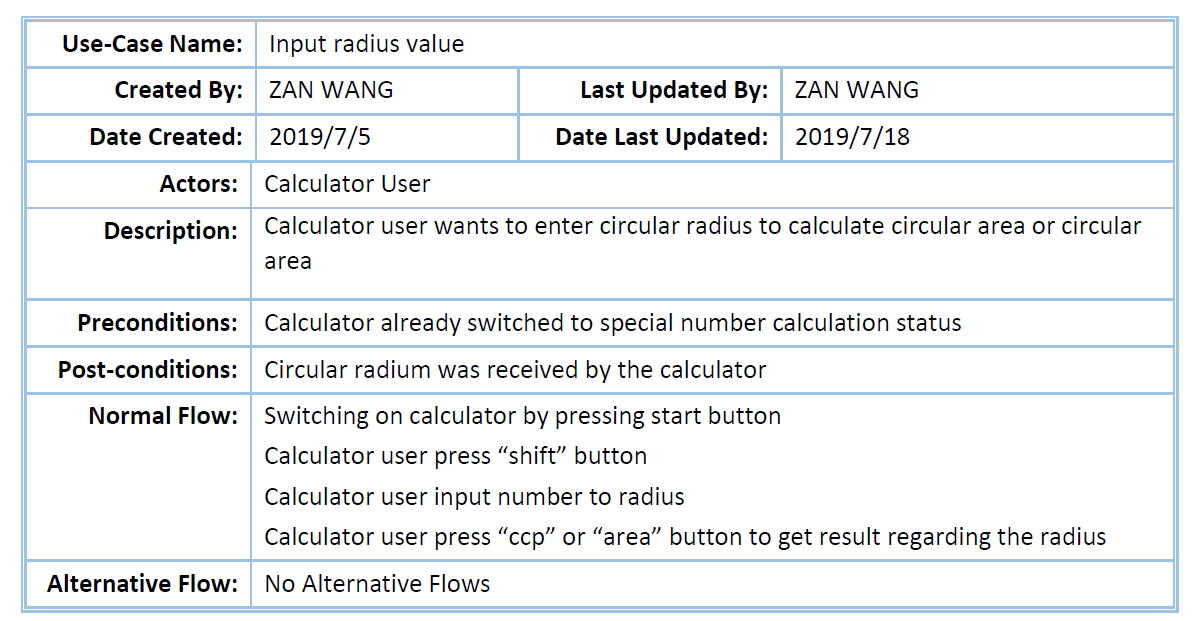
\includegraphics[width=0.915\textwidth]{images/use_case/UC_irv.PNG}
\end{figure}

\begin{figure}[H]
\centering  %图片全局居中
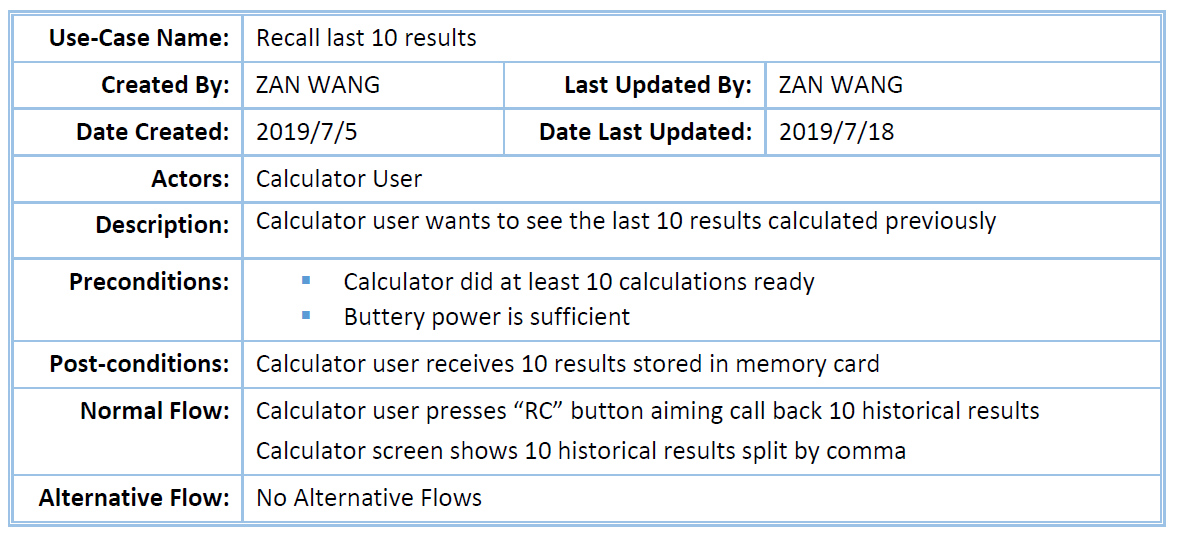
\includegraphics[width=0.9\textwidth]{images/use_case/UC_rl10r.PNG}
\end{figure}



\section{Sequence Diagram for Main Use Cases}

\begin{figure}[H]
\centering  %图片全局居中
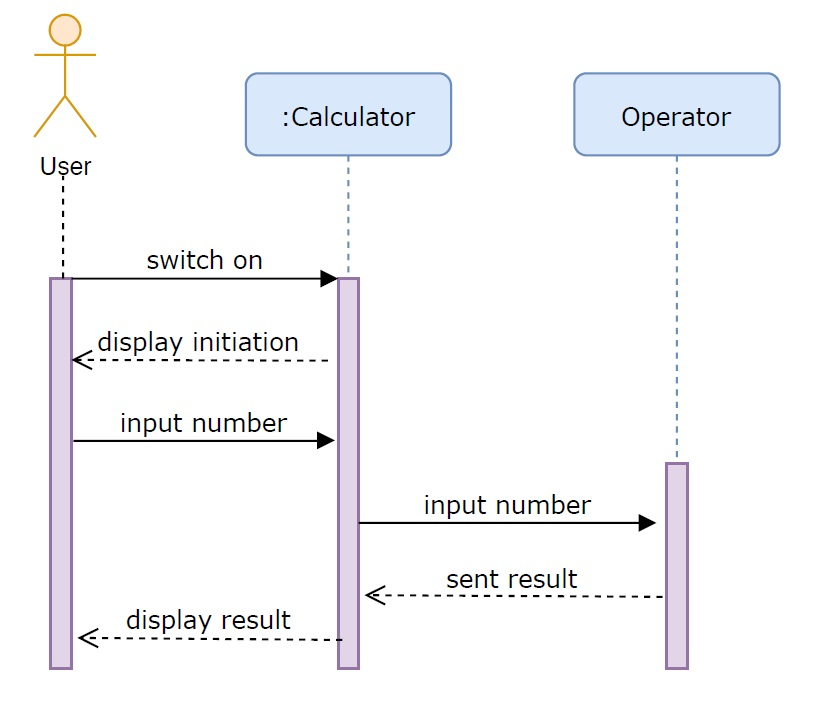
\includegraphics[width=0.6\textwidth]{images/SD/ccn.jpg}
\caption{Input Regular Number}
\end{figure}

\begin{figure}[H]
\centering  %图片全局居中
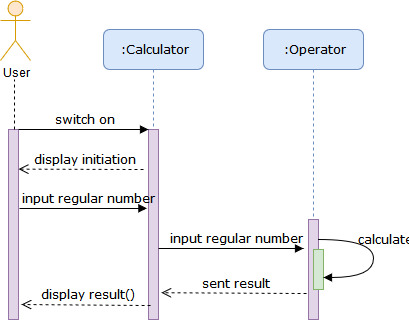
\includegraphics[width=0.6\textwidth]{images/SD/irn.jpg}
\caption{Calculate Regular Number}
\end{figure}

\begin{figure}[H]
\centering  %图片全局居中
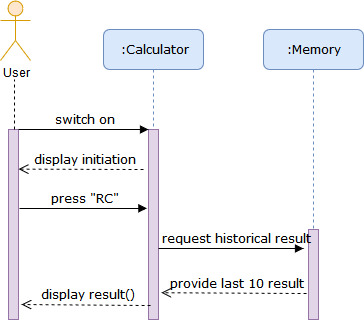
\includegraphics[width=0.6\textwidth]{images/SD/rl10r.jpg}
\caption{Recollect Historical Result}
\end{figure}

\begin{figure}[H]
\centering  %图片全局居中
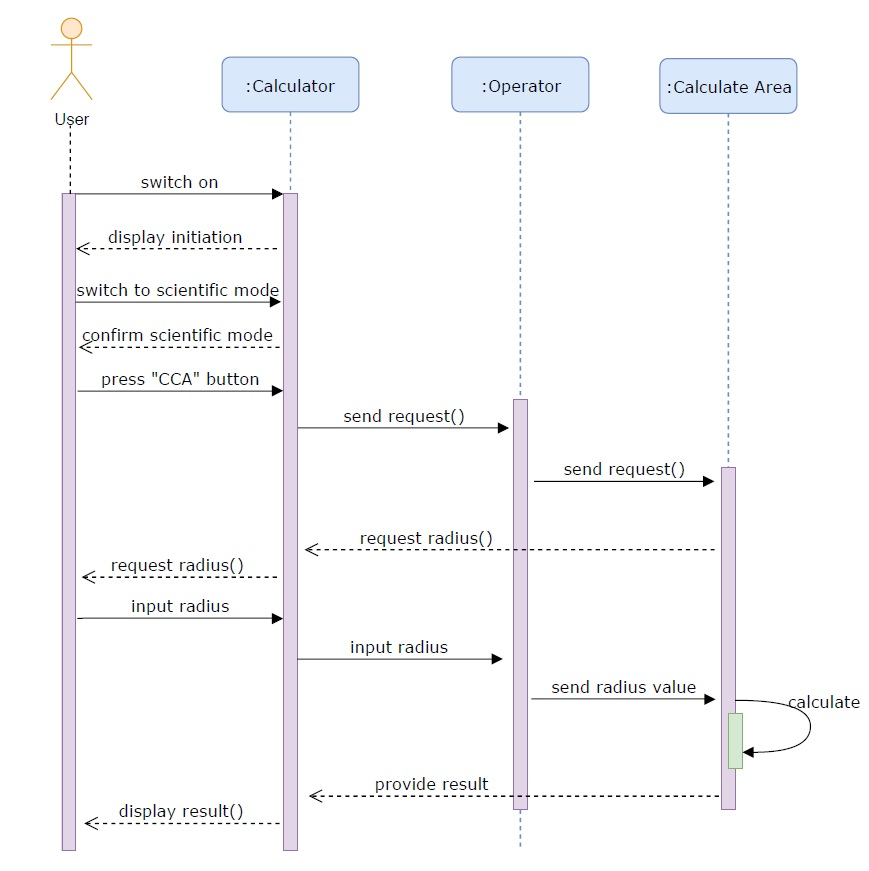
\includegraphics[width=0.7\textwidth]{images/SD/cca.jpg}
\caption{Calculate Circular Area}
\end{figure}

\begin{figure}[H]
\centering  %图片全局居中
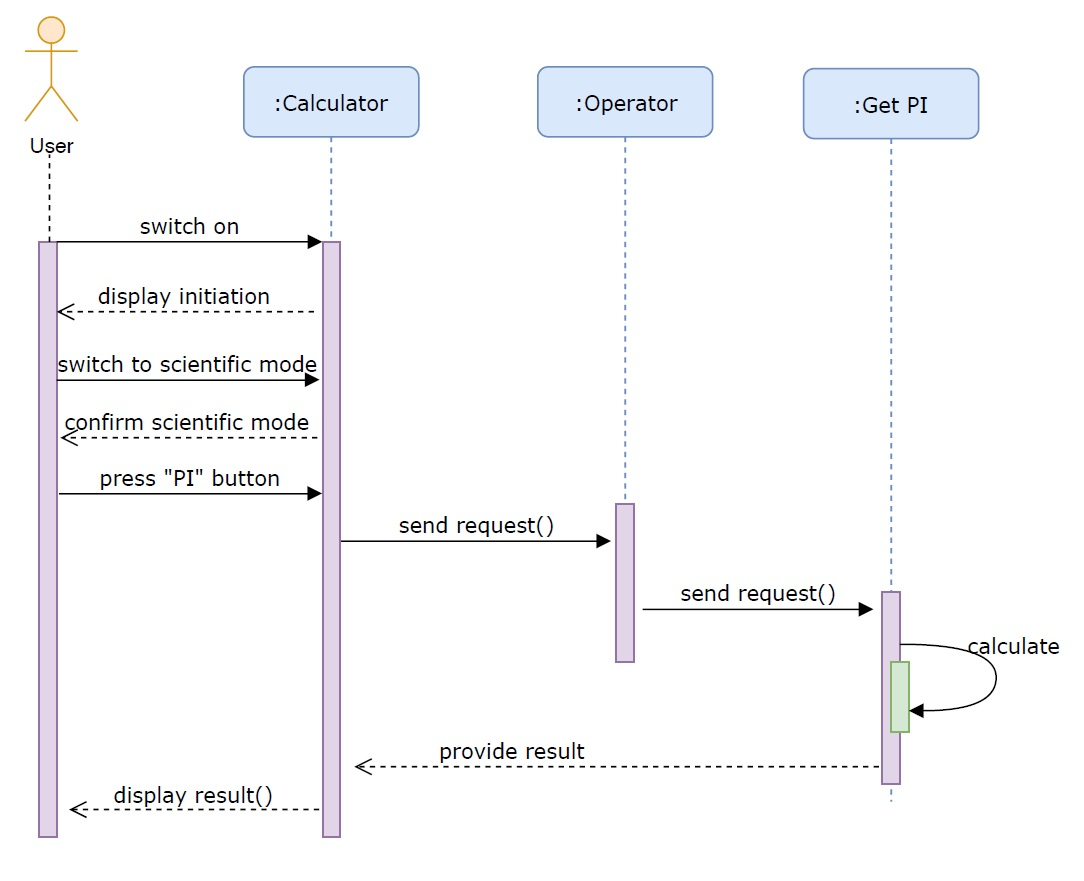
\includegraphics[width=0.6\textwidth]{images/SD/getpi.jpg}
\caption{Calculate PI}
\end{figure}

\begin{figure}[H]
\centering  %图片全局居中
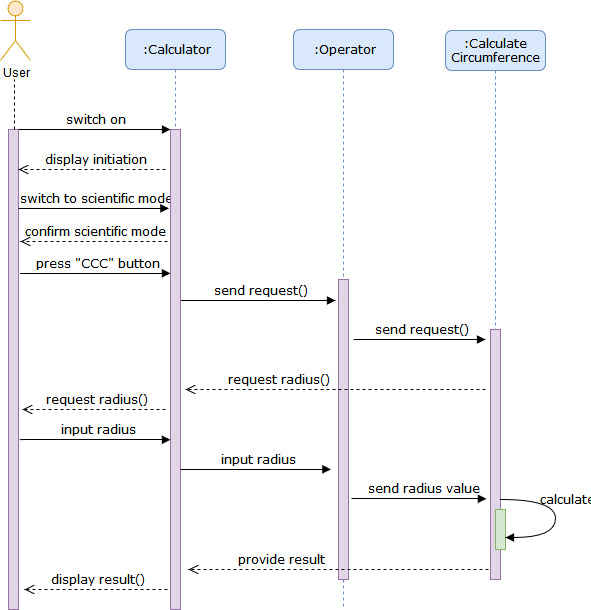
\includegraphics[width=0.6\textwidth]{images/SD/ccc.jpg}
\caption{Calculate Circular Circumference}
\end{figure}



\vspace{50pt}
\section{Activity Diagram}

\begin{flushleft}
\vspace{8pt}
\noindent
Activity Diagrams describe how activities are coordinated to provide a calculation results which can be at different levels of abstraction. Typically, user needs to switch on the calculator first, then the user could choose to trace the last 10 results, calculate regular number, or calculate special scientific number (PI). If user want to have scientific number, then functions related to this scientific number could be applied. Taking PI as an example, addition to get the PI value, user also can know circular area and circular circumference after inputting exact radius value for intended circular.
\end{flushleft}


\begin{figure}[H]
\centering  %图片全局居中
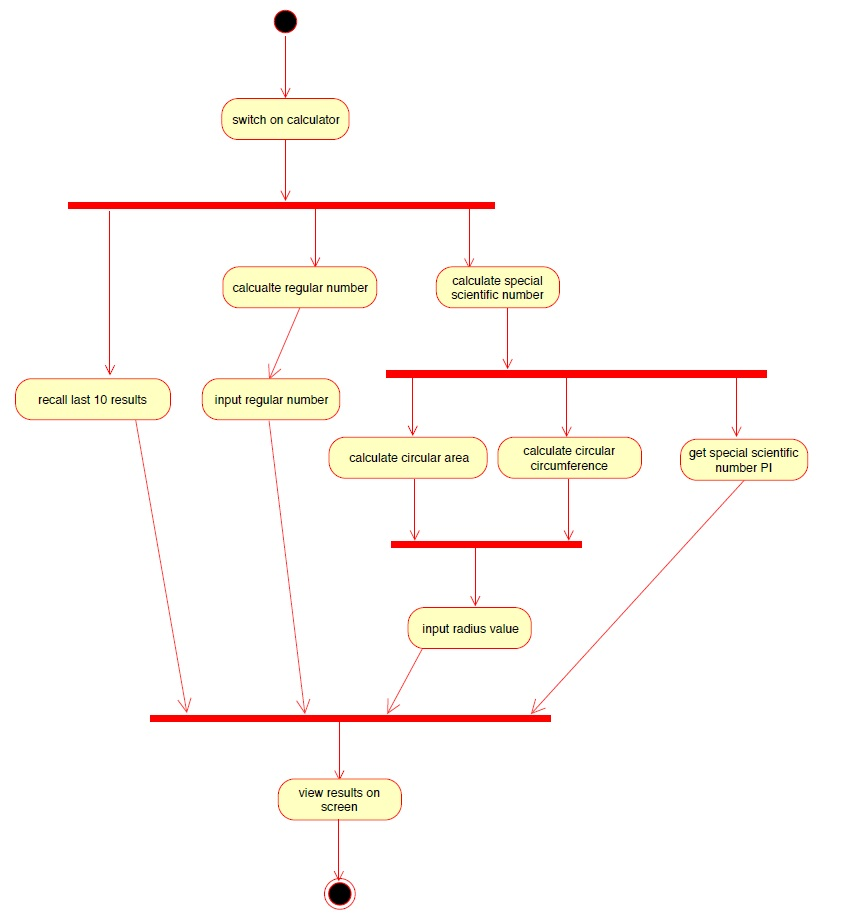
\includegraphics[width=0.8\textwidth]{images/activity_diagram.jpg}
\caption{Activity Diagram}
\end{figure}





%\bibliography{AdminTechII} % Archivo de bibliografía bib
%\bibliographystyle{apalike} % Estilo APA 6

% apendices

\end{document}
